
%
%===================================================================================================
% Universidade: Universidade Federal de Goiás - UFG
% Curso.......: Ciência da Computação - BCC
% Disciplina..: Estruturas de Dados - 1
% Ano/Semestre: 2017/2
%
% Professor...: Wanderley de Souza Alencar
%
% Alunos: Luigi Wagner, Rafael Alessandro e Rafael Falcão.
%
% Material....: Modelo de Slides para Apresentação de Seminário
%
%===================================================================================================
%
\documentclass[cyan,compress,aspectratio=43]{beamer}
\definecolor{mycolor}{rgb}{.0,.545,.545}
\usecolortheme[named=mycolor]{structure}
%\usepackage[dvips]{graphicx}            % to include images
\usepackage[english,portuguese,brazil]{babel}
%\usepackage[T1]{fontenc} 
%\usepackage[ansinew]{inputenc} 
\usepackage[utf8x]{inputenc}  
\usepackage{graphicx}
\usepackage{longtable}
\usepackage{float}
\usepackage{fancyvrb}
\usepackage{amsfonts}
\usepackage{amsmath}
\usepackage{amssymb}
\usepackage{url}
%\usepackage[vlined,titlenumbered,algo2e,ruled]{algorithm2e} 
\usepackage[english, ruled, vlined, longend]{algorithm2e}
\usepackage{indentfirst}
\usepackage{subfigure}
\usepackage{color}
%\usepackage{times}
\usepackage{listings}
\definecolor{listinggray}{gray}{0.9}
\definecolor{lbcolor}{rgb}{0.9,0.9,0.9}
\lstset{
    language=c,
    basicstyle=\scriptsize,
    upquote=true,
    aboveskip={0.1\baselineskip},
    columns=fullflexible,
    showstringspaces=false,
    numbers=left,
    numberstyle=\tiny\color{gray},
    stepnumber=1,
    numbersep=5pt, 
    extendedchars=true,
    breaklines=true,
    showtabs=false,
    showspaces=false,
    identifierstyle=\ttfamily,
    keywordstyle=\color[rgb]{0,0,1},
    commentstyle=\color[rgb]{0.133,0.545,0.133},
    stringstyle=\color[rgb]{0.627,0.126,0.941},
    tabsize=3,
}

\usetheme{Warsaw}
\usefonttheme{professionalfonts}
\usenavigationsymbolstemplate{}
\title{Árvore 2-3}


\author[Luigi, Rafael A. e Rafael F.]{ Luigi Wagner \\ Rafael Alessandro \\ Rafael Falcão
}
\institute{
        Ciências da Computação -- Disciplina: Estruturas de Dados -- 1 \\
	Instituto de Informática \\
	Universidade Federal de Goiás
}

\date{\today}

\AtBeginSection[]
{
 \begin{frame}<beamer>
  \frametitle{Sumário}
  \tableofcontents[currentsection]
 \end{frame}
}

%INSERIR NÚMERO DA PÁGINA
\expandafter\def\expandafter\insertshorttitle\expandafter{%
  \insertshorttitle\hfill%
  \insertframenumber\,/\,\inserttotalframenumber
}

\begin{document}
\frame{\titlepage}
%
%---------------------------------------------------------------------------------------------------
% Primeiro Tópico
%---------------------------------------------------------------------------------------------------
%
\section[\thesection]{Introdução}

\frame { \frametitle{Introdução}
    Uma Árvore 2-3 é uma árvore onde cada nó com filho (nó interno) tem também 2 filhos (2-node) e 1 elemento de dados (chave) ou 3 filhos (3-nodes) e 2 elementos de dados (chaves).
Os nós externos a árvore (nós-folha) não tem filhos e possuem um ou dois elementos de dados (chaves).
}

%\frame { \frametitle{Introdução}
%	Cada \texttt{seção} (ou \emph{section}, em LaTeX) deve corresponder a um dos tópicos a serem abordados naquele tema.
%	\newline
%	\newline
%	As \texttt{seções} podem, livremente, serem subdividas em subseções e subsubseções.
%}

\frame { \frametitle{Introdução}
	\begin{block}{Propriedades}
		As principais \texttt{propriedades} de uma Árvore 2-3 são:
		%\newline
		\newline
		\begin{itemize}
		      \item Cada nó interno tem dois filhos (2-node) se tem uma chave, ou três filhos (3-node) se tem duas chaves; 
		      \item Cada nó não-folha tem 2 ou 3 filhos. Se tem 2 filhos tem 1 item de dados e se tem 3 filhos tem 2 itens de dados;
		      \item Todos os dados são ordenados;
		      \item Todas as folhas estão no mesmo nível- assim como na Árvore B;
		      \item Cada nó folha tem 1 ou 2 campos.
		      %\item $\dots$
		\end{itemize}
        Como, por exemplo:
	\end{block}
}

\frame { \frametitle{Introdução}
	\begin{figure}[htbp]
		\centering
		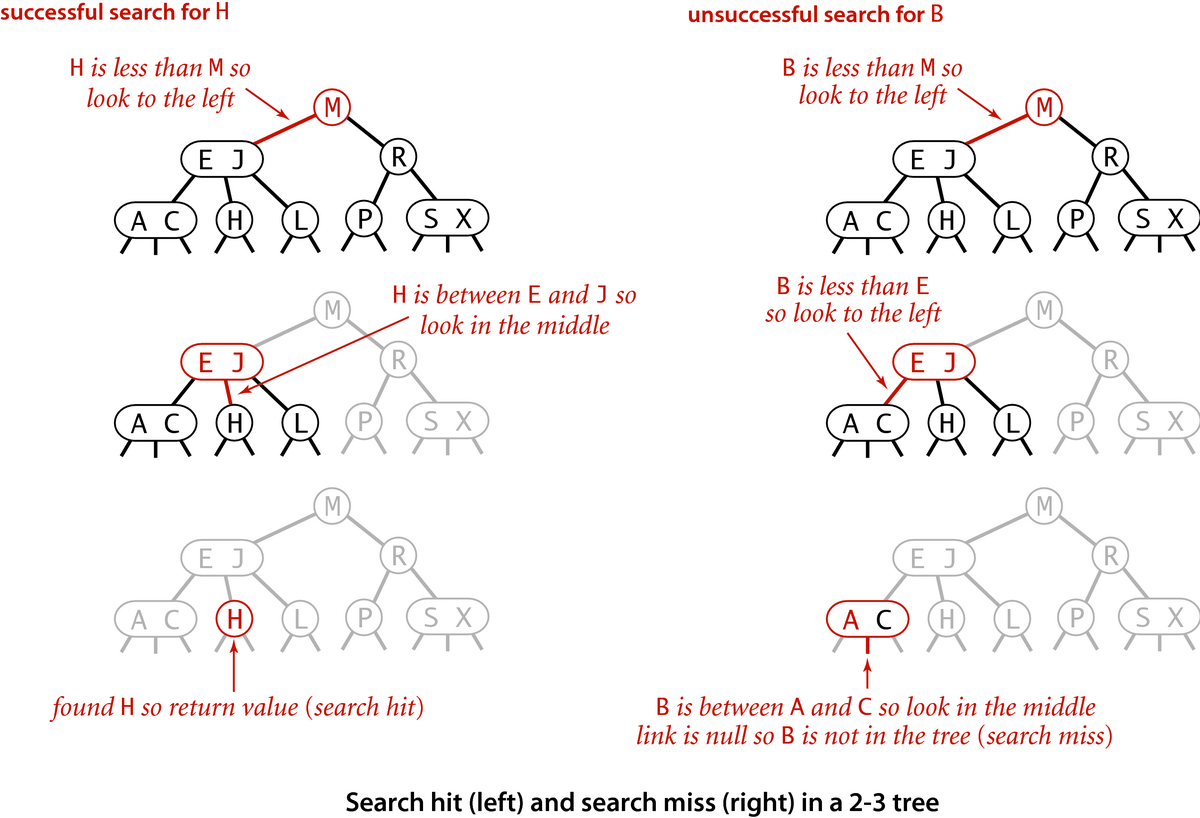
\includegraphics[width=.8\textwidth]{./fig/23tree2.png}	
		\caption{\url{https://www.ime.usp.br/~pf/estruturas-de-dados/aulas/figuressw/Chapter3/TTsearch.png}}
        \end{figure}
}

% $\mathcal{L}$ << FICA MAIS COOL A LETRA

\frame { \frametitle{Introdução}
	\begin{block}{\textit{Componentes ou Anatomia}}
		Uma Árvore 2-3 é composta por:
		\begin{enumerate}
		      \item Componente 1;
		      \item Componente 2;
		      \item Componente 3.
		\end{enumerate}
	\end{block}
	\begin{figure}[htbp]
		\centering
		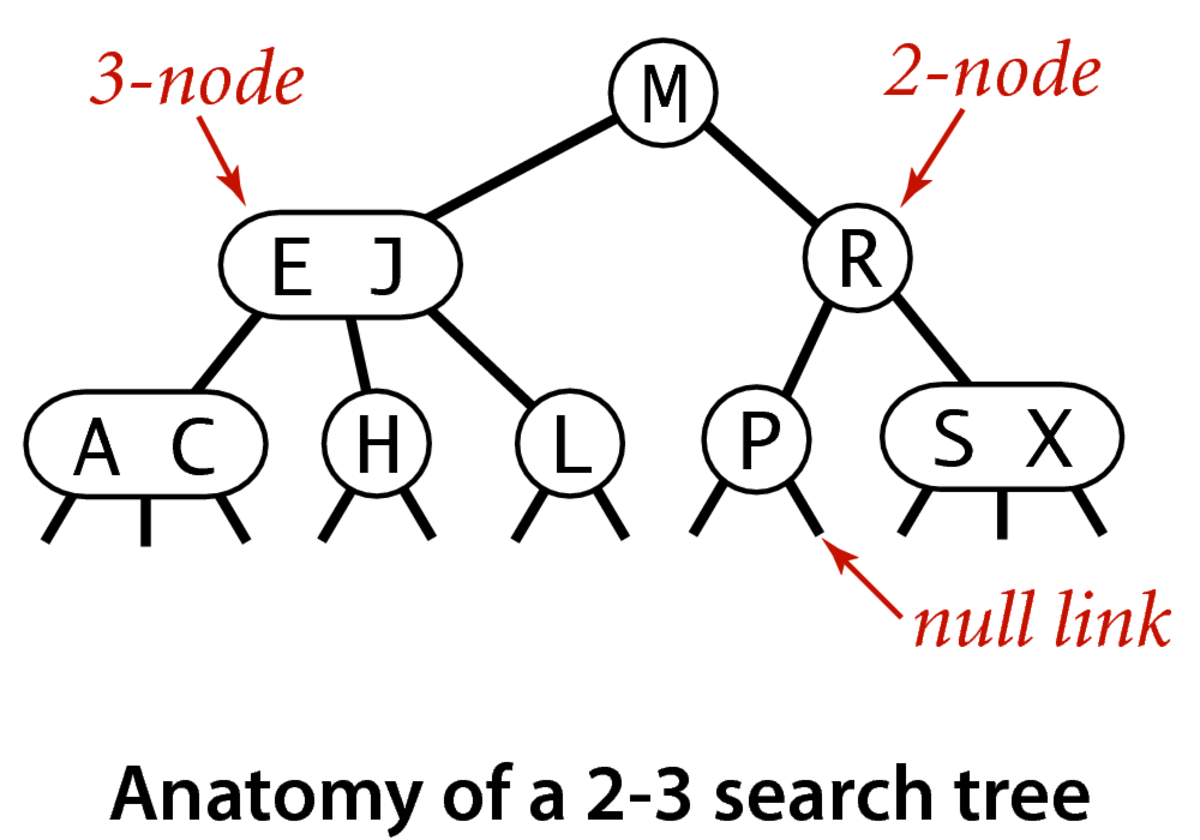
\includegraphics[width=0.4\textwidth]{./fig/23tree.png}
		\caption{\url{https://www.ime.usp.br/~pf/estruturas-de-dados/aulas/figuressw/Chapter3/TTanatomy.png}}
        \end{figure}
}

\frame { \frametitle{Introdução}
	\begin{block}{Bloco}
		Um \texttt{bloco} pode conter figuras, tabelas, listas, etc.
	\end{block}
	
}

%
%---------------------------------------------------------------------------------------------------
% Pesquisa
%---------------------------------------------------------------------------------------------------
%
\section[\thesection]{Pesquisa}

\frame { \frametitle{Pesquisa em uma Árvore 2-3}
	\begin{block}{}
		Vamos começar pelo mais básico procedimento a ser realizado
		ao lidar com uma \color{blue}{Árvore}.
	\end{block}
	
}
\frame { \frametitle{Pesquisa em uma Árvore 2-3}
	Exemplo de uma Árvore 2-3
	\begin{figure}[htbp]
		\centering
		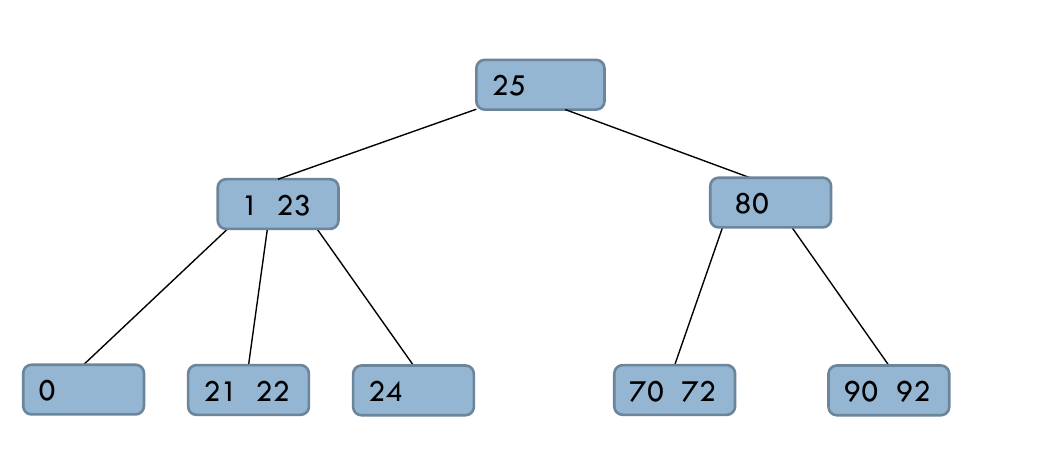
\includegraphics[width=1\textwidth]{./fig/23tree3.png}	
		\caption{Imagem retirada de [2] (vide \textit{Referências Bibliográficas})}
        \end{figure}
}
\frame { \frametitle{Pesquisa em uma Árvore 2-3}
	Pesquisando pela chave 72 na Árvore:
	\begin{figure}[htbp]
		\centering
		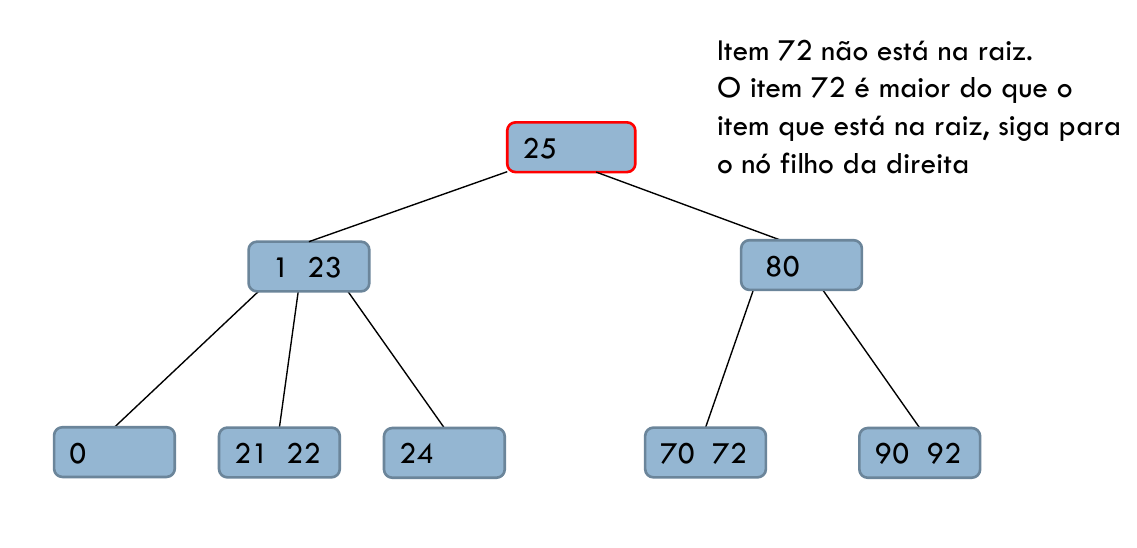
\includegraphics[width=1\textwidth]{./fig/23tree4.png}	
		\caption{Imagem retirada de [2] (vide \textit{Referências Bibliográficas})}
        \end{figure}
}
\frame { \frametitle{Pesquisa em uma Árvore 2-3}
	Pesquisando pela chave 72 na Árvore:
	\begin{figure}[htbp]
		\centering
		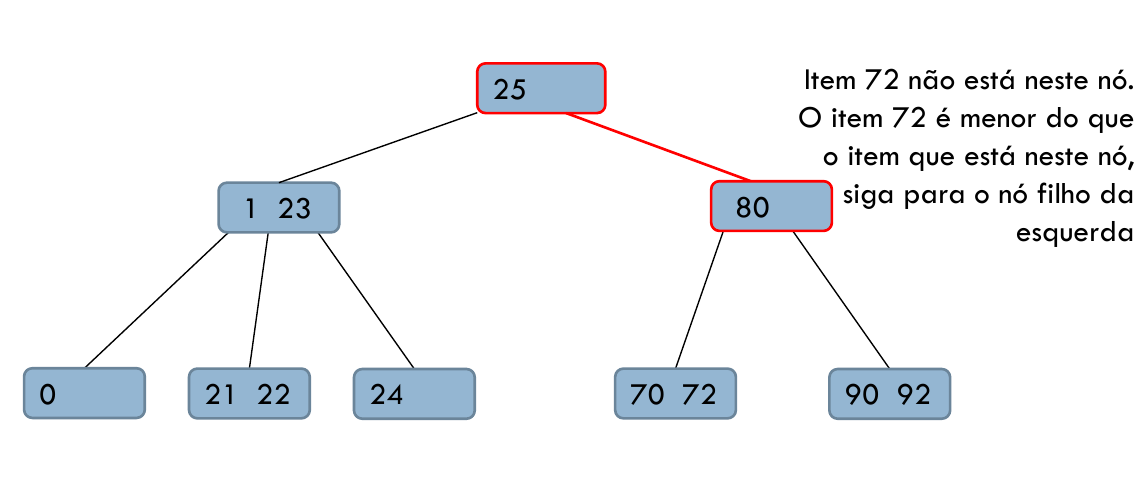
\includegraphics[width=1\textwidth]{./fig/23tree5.png}	
		\caption{Imagem retirada de [2] (vide \textit{Referências Bibliográficas})}
        \end{figure}
}
\frame { \frametitle{Pesquisa em uma Árvore 2-3}
	Pesquisando pela chave 72 na Árvore:
	\begin{figure}[htbp]
		\centering
		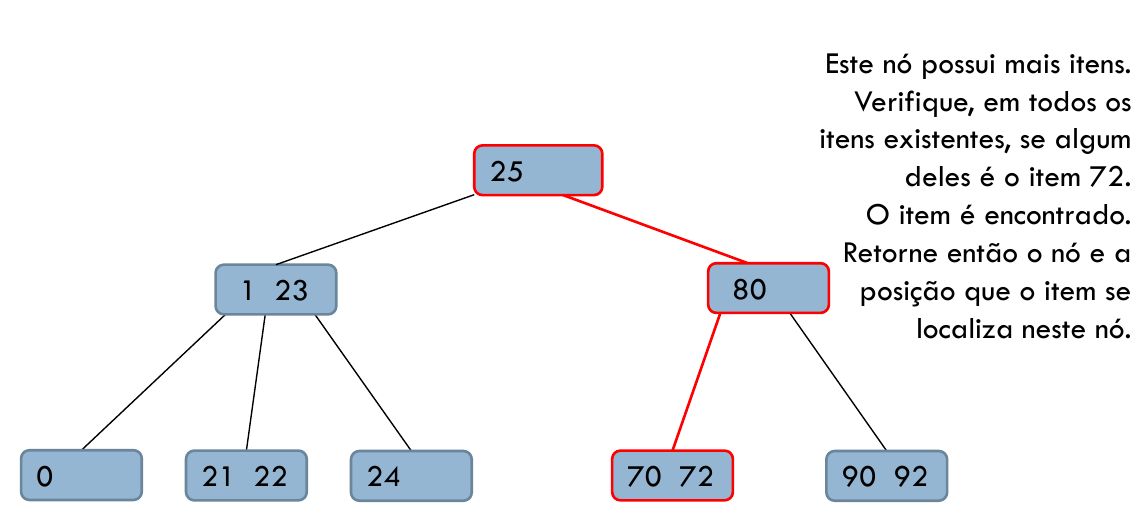
\includegraphics[width=1\textwidth]{./fig/23tree6.png}	
		\caption{Imagem retirada de [2] (vide \textit{Referências Bibliográficas})}
        \end{figure}
}
%
%---------------------------------------------------------------------------------------------------
% Inserção
%---------------------------------------------------------------------------------------------------
%
\section[\thesection]{Inserção}

\frame { \frametitle{Inserção em uma Árvore 2-3}
	\begin{block}{}
		Continuando os procedimentos, vamos à \textit{Inserção} em uma \color{blue}{Árvore 2-3}.
	\end{block}
	
}
\frame { \frametitle{Inserção em uma Árvore 2-3}
	Inserindo a chave 50 na Árvore:
	\begin{figure}[htbp]
		\centering
		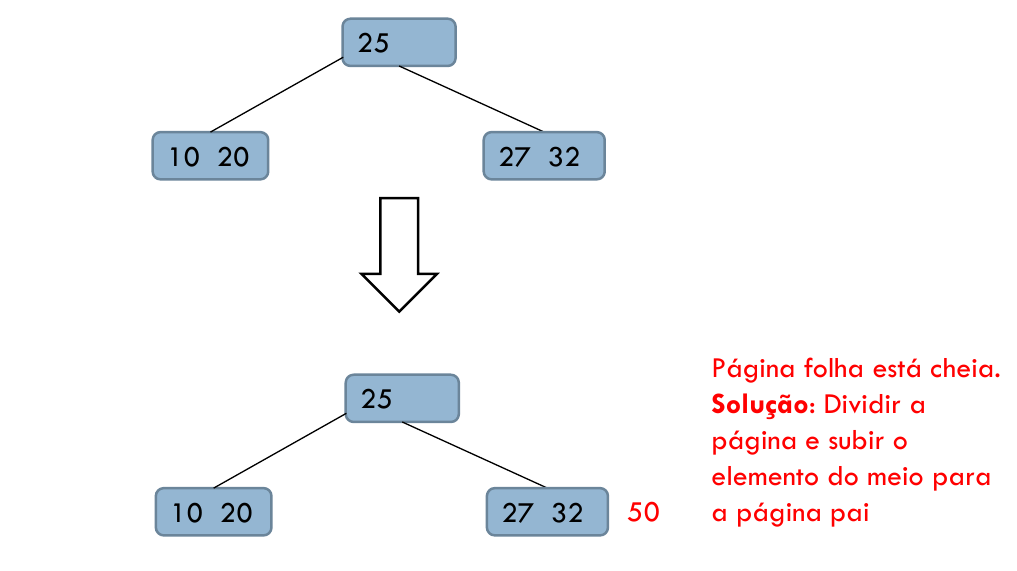
\includegraphics[width=1\textwidth]{./fig/23tree7.png}	
		\caption{Imagem retirada de [2] (vide \textit{Referências Bibliográficas})}
        \end{figure}
}
\frame { \frametitle{Inserção em uma Árvore 2-3}
	Inserindo a chave 50 na Árvore:
	\begin{figure}[htbp]
		\centering
		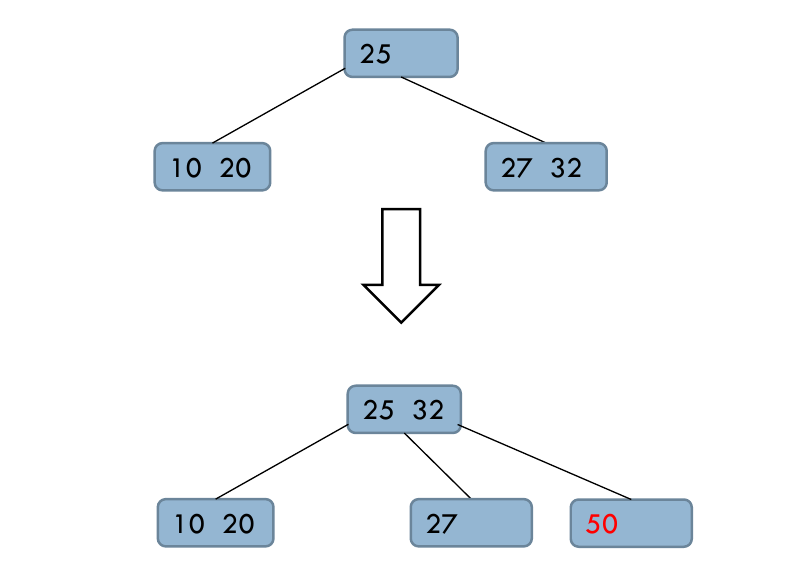
\includegraphics[width=.8\textwidth]{./fig/23tree8.png}	
		\caption{Imagem retirada de [2] (vide \textit{Referências Bibliográficas})}
        \end{figure}
}
\frame { \frametitle{Inserção em uma Árvore 2-3}
	Inserindo a chave 5 na Árvore:
	\begin{figure}[htbp]
		\centering
		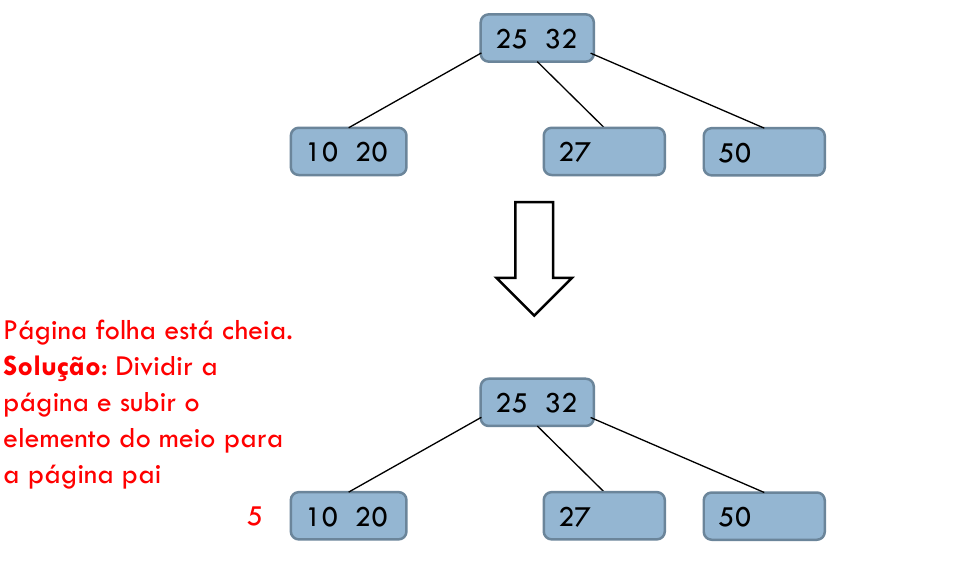
\includegraphics[width=.9\textwidth]{./fig/23tree9.png}	
		\caption{Imagem retirada de [2] (vide \textit{Referências Bibliográficas})}
        \end{figure}
}
\frame { \frametitle{Inserção em uma Árvore 2-3}
	Inserindo a chave 5 na Árvore:
	\begin{figure}[htbp]
		\centering
		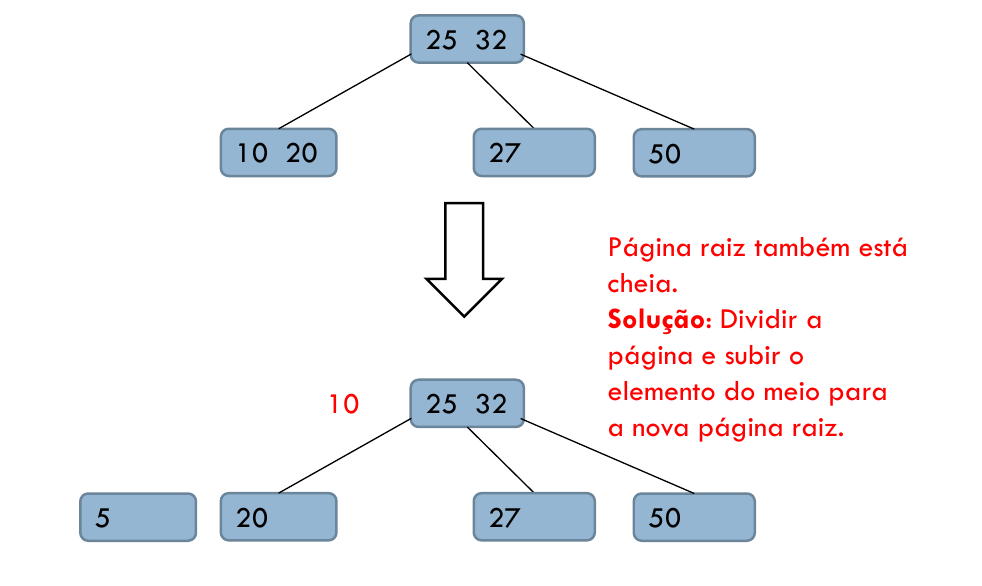
\includegraphics[width=.9\textwidth]{./fig/23tree10.png}	
		\caption{Imagem retirada de [2] (vide \textit{Referências Bibliográficas})}
        \end{figure}
}
\frame { \frametitle{Inserção em uma Árvore 2-3}
	Inserindo a chave 5 na Árvore:
	\begin{figure}[htbp]
		\centering
		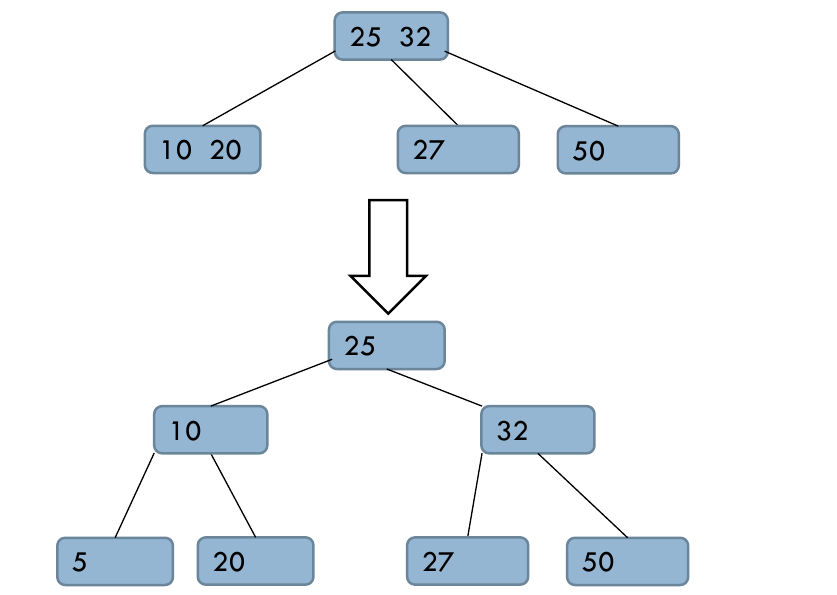
\includegraphics[width=.7\textwidth]{./fig/23tree11.png}	
		\caption{Imagem retirada de [2] (vide \textit{Referências Bibliográficas})}
        \end{figure}
}

%
%---------------------------------------------------------------------------------------------------
% Remoção
%---------------------------------------------------------------------------------------------------
%
\section[\thesection]{Remoção}

\frame { \frametitle{Remoção em uma Árvore 2-3}
	\begin{block}{}
		Hora de tratarmos do mais complexo dos procedimentos relacionados à uma
		\textit{Árvore 2-3}, a Remoção.
	\end{block}
	
}
\frame { \frametitle{Remoção em uma Árvore 2-3}
	Começaremos pelo mais simples:
	\newline
	Exemplo 1:
	%item 73
	\begin{figure}[htbp]
		\centering
		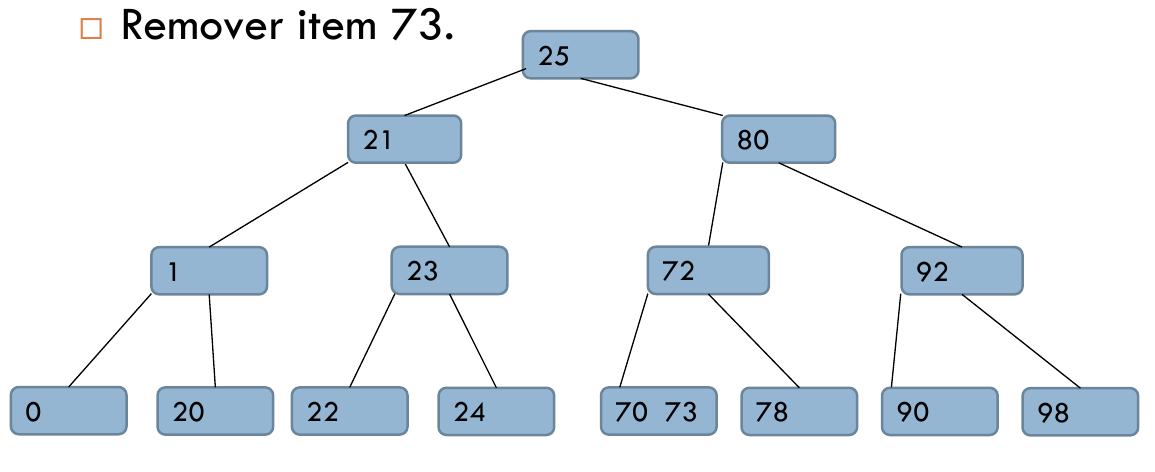
\includegraphics[width=1\textwidth]{./fig/23tree12.png}	
		\caption{Imagem retirada de [2] (vide \textit{Referências Bibliográficas})}
        \end{figure}
}
\frame { \frametitle{Remoção em uma Árvore 2-3}
	%item 73
	\begin{figure}[htbp]
		\centering
		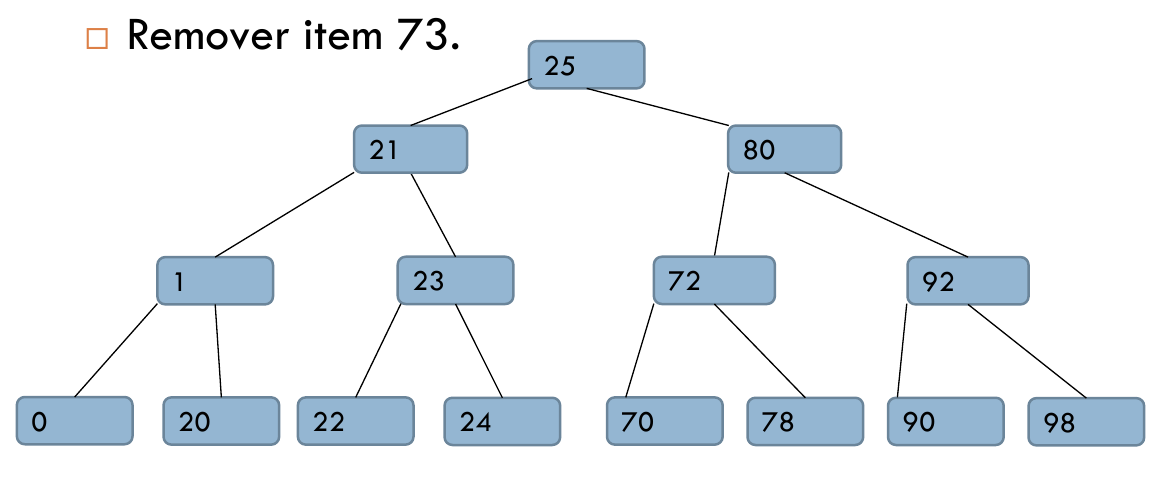
\includegraphics[width=1\textwidth]{./fig/23tree13.png}	
		\caption{Imagem retirada de [2] (vide \textit{Referências Bibliográficas})}
        \end{figure}
}
\frame { \frametitle{Remoção em uma Árvore 2-3}
	%item 20
	Exemplo 2:
	\begin{figure}[htbp]
		\centering
		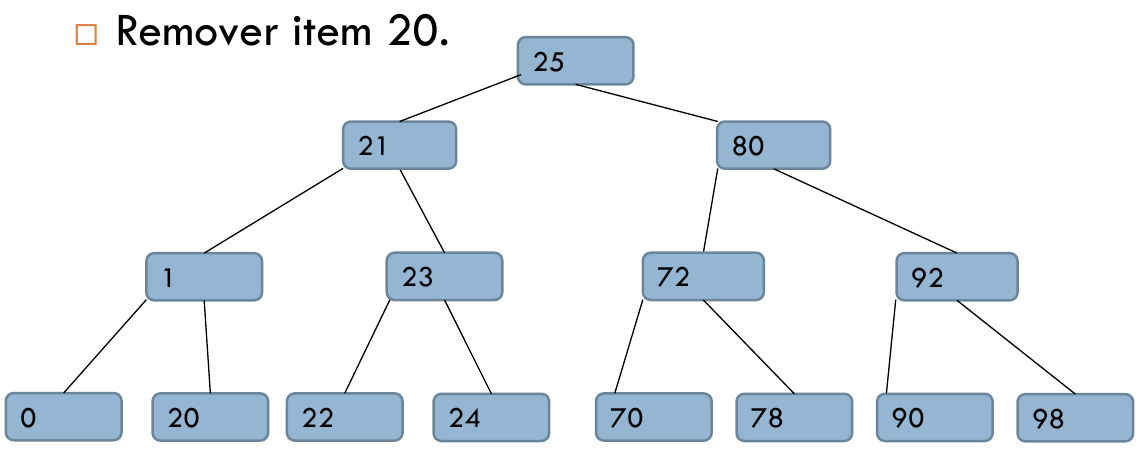
\includegraphics[width=1\textwidth]{./fig/23tree14.png}	
		\caption{Imagem retirada de [2] (vide \textit{Referências Bibliográficas})}
        \end{figure}
}
\frame { \frametitle{Remoção em uma Árvore 2-3}
	\begin{block}{Problema!}
	    \textit{Houston, we have a problem.}
	    \newline
		Repare que não podemos remover diretamente o 20, temos que reorganizar a Árvore
		para manter suas propriedades válidas.
		\newline
		No caso, a propriedade referida é a de um nó ter 2 ou três filhos, não é permitido
		apenas um filho.
	\end{block}
}
\frame { \frametitle{Remoção em uma Árvore 2-3}
	\begin{figure}[htbp]
		\centering
		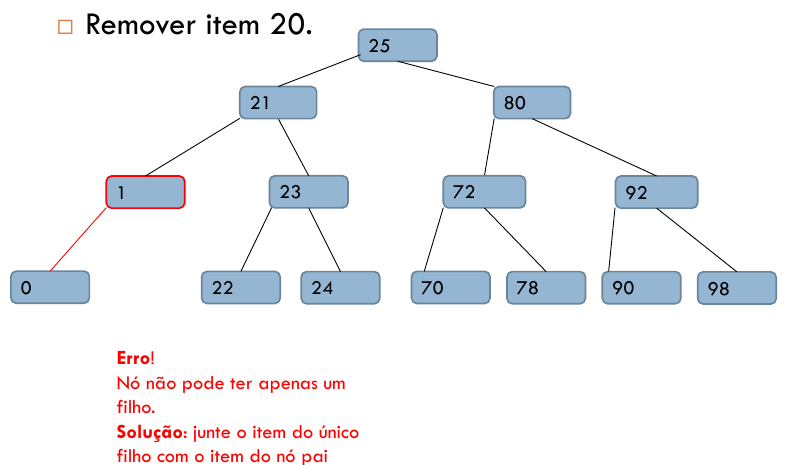
\includegraphics[width=1\textwidth]{./fig/23tree15.png}	
		\caption{Imagem retirada de [2] (vide \textit{Referências Bibliográficas})}
        \end{figure}
}
\frame { \frametitle{Remoção em uma Árvore 2-3}
	\begin{figure}[htbp]
		\centering
		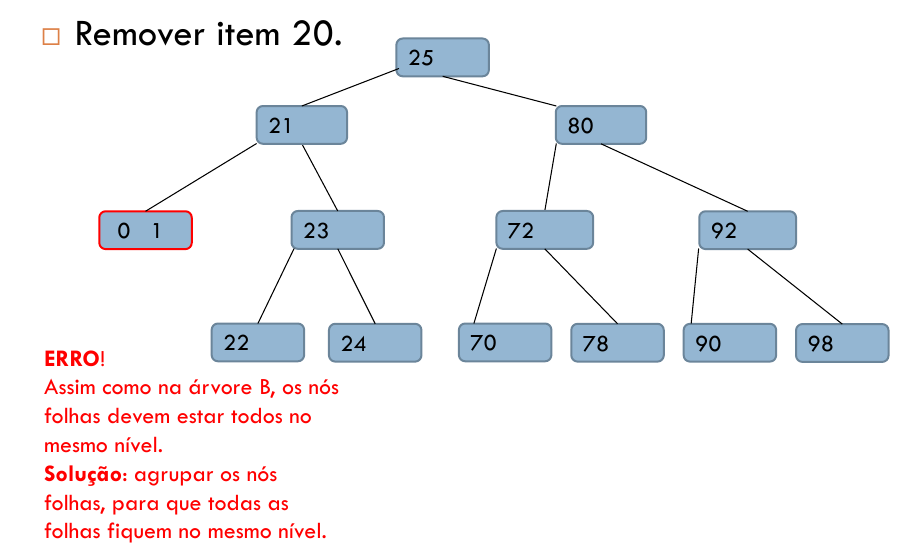
\includegraphics[width=1\textwidth]{./fig/23tree16.png}	
		\caption{Imagem retirada de [2] (vide \textit{Referências Bibliográficas})}
        \end{figure}
}
\frame { \frametitle{Remoção em uma Árvore 2-3}
	\begin{figure}[htbp]
		\centering
		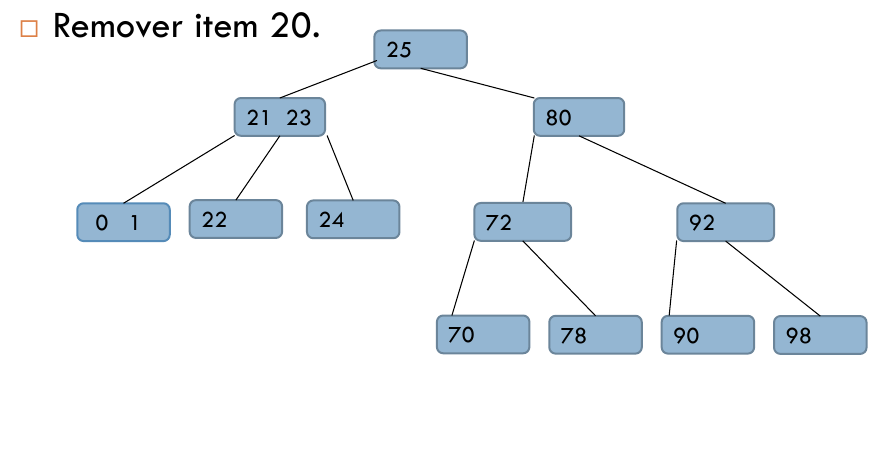
\includegraphics[width=1\textwidth]{./fig/23tree17.png}	
		\caption{Imagem retirada de [2] (vide \textit{Referências Bibliográficas})}
        \end{figure}
}
\frame { \frametitle{Remoção em uma Árvore 2-3}
	\begin{figure}[htbp]
		\centering
		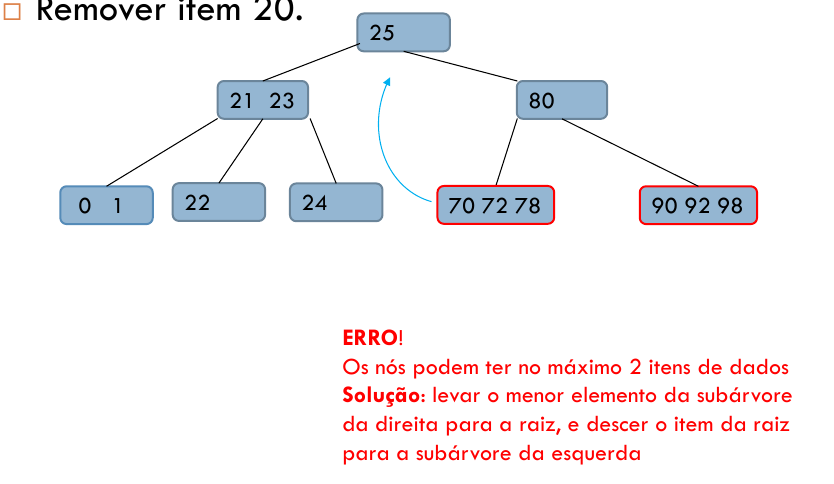
\includegraphics[width=1\textwidth]{./fig/23tree18.png}	
		\caption{Imagem retirada de [2] (vide \textit{Referências Bibliográficas})}
        \end{figure}
}
\frame { \frametitle{Remoção em uma Árvore 2-3}
	\begin{figure}[htbp]
		\centering
		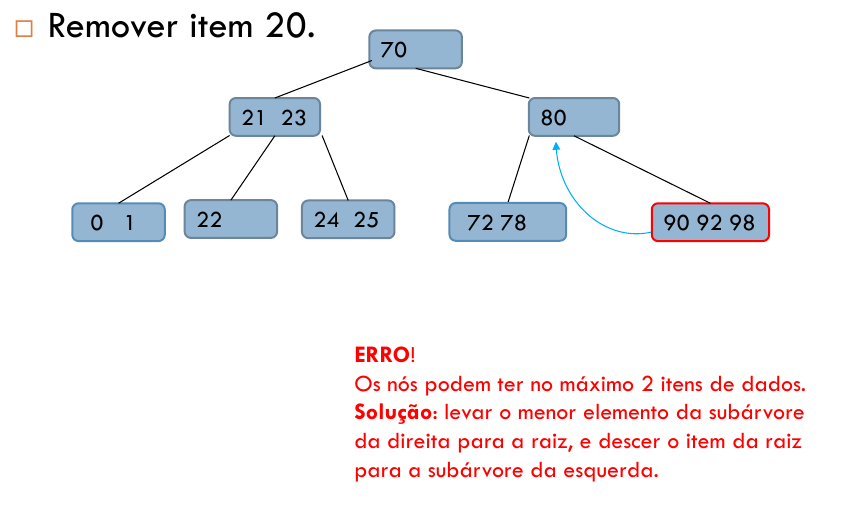
\includegraphics[width=1\textwidth]{./fig/23tree19.png}	
		\caption{Imagem retirada de [2] (vide \textit{Referências Bibliográficas})}
        \end{figure}
}
\frame { \frametitle{Remoção em uma Árvore 2-3}
	\begin{figure}[htbp]
		\centering
		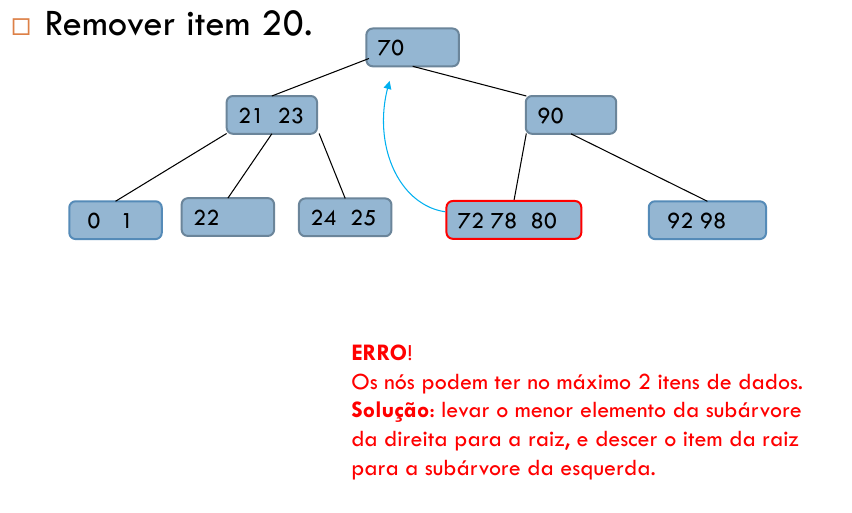
\includegraphics[width=1\textwidth]{./fig/23tree20.png}	
		\caption{Imagem retirada de [2] (vide \textit{Referências Bibliográficas})}
        \end{figure}
}
\frame { \frametitle{Remoção em uma Árvore 2-3}
	\begin{figure}[htbp]
		\centering
		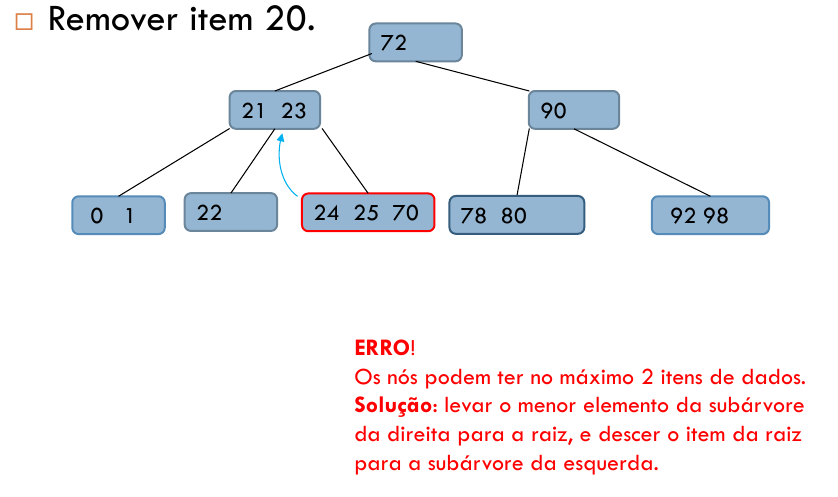
\includegraphics[width=1\textwidth]{./fig/23tree21.png}	
		\caption{Imagem retirada de [2] (vide \textit{Referências Bibliográficas})}
        \end{figure}
}
\frame { \frametitle{Remoção em uma Árvore 2-3}
	\begin{figure}[htbp]
		\centering
		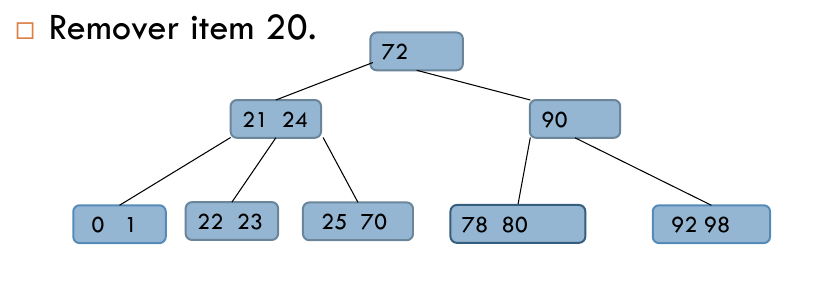
\includegraphics[width=1\textwidth]{./fig/23tree22.png}	
		\caption{Imagem retirada de [2] (vide \textit{Referências Bibliográficas})}
        \end{figure}
}
\frame { \frametitle{Remoção em uma Árvore 2-3}
	\begin{figure}[htbp]
		\centering
		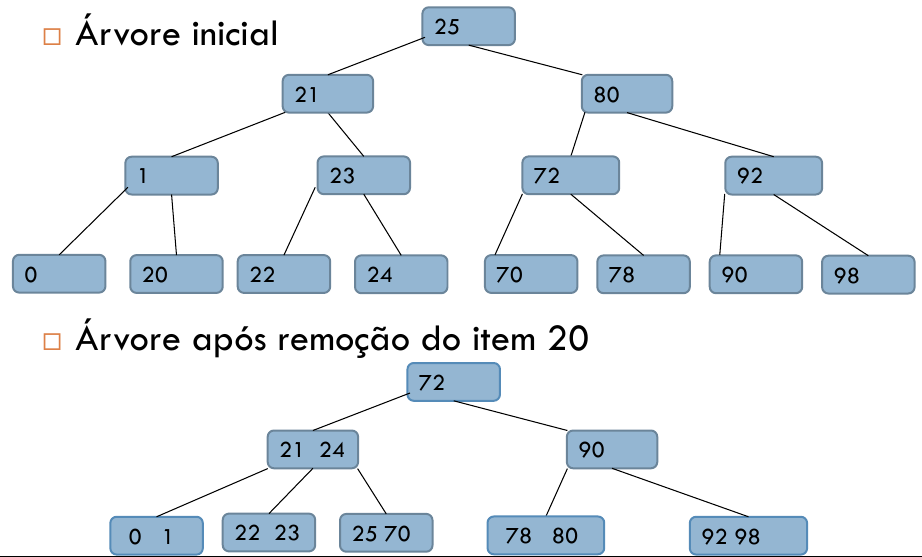
\includegraphics[width=1\textwidth]{./fig/23tree23.png}	
		\caption{Imagem retirada de [2] (vide \textit{Referências Bibliográficas})}
        \end{figure}
}

 \frame { \frametitle{Remoção em uma Árvore 2-3}
 	\begin{block}{}
 	    Entenderam o porquê do \textit{complexo} agora, ou seja, tenham plena certeza de suas inserções
	    ou sofrerão com sua remoção!
 	\end{block}
}

 
 %
%---------------------------------------------------------------------------------------------------
% Segundo Tópico
%---------------------------------------------------------------------------------------------------
%
\section[\thesection]{Códigos}

%\frame { \frametitle{Acerca dos código}
%	Aqui começamos um segundo tópico, ou seja, a segunda seção dos \emph{slides}
%	\begin{itemize}
%	 	\item Operações sobre linguagens;
%	 	\item Expressões regulares.
%	\end{itemize}
%}


%\frame { \frametitle{Segundo Tópico}
%	\begin{block}{Matemático}
%		Um \emph{slide} pode utilizar símbolos matemáticos, como:
%		\begin{itemize}
%   		\item $\epsilon$ é uma letra grega que normalmente denota quantidades extremamente pequenas; 
%    		\item $\alpha$, $\beta$, e $\gamma$ são outras letras gregas.
%   		\end{itemize}
%	\end{block}
%}

\frame { \frametitle{}
	\begin{block}{Programas}
		Agora que já vimos como funciona e os princípios básicos
		das  \textcolor{blue}{Árvores 2-3}, daremos uma olhada nas \texttt{estruturas} e \texttt{algoritmos} para a manipulação
		e armazenamento das supracitadas \textcolor{blue}{Árvores 2-3}.
		\begin{enumerate}
		      \item Estrutura básica (\textcolor{blue}{Struct});
		      \item Alocação da \textcolor{blue}{Árvore 2-3}.
		\end{enumerate}

	\end{block}
}

\begin{frame}[fragile]
\frametitle{Código}
  \vspace{-0.3cm}
  \begin{block}{Estrutura de uma Árvore 2-3}
     	\begin{lstlisting}
	  typedef struct _no23 {
	    int	lkey,             // chave esquerda
		    rkey,             // chave direita
		    nkeys;            // numero de chaves
	    struct _no23	*left,    // ponteiro ao filho esquerdo 
				    *center,  // ponteiro ao filho central
				    *right;   // ponteiro ao filho direito
	  } no23;   
    	\end{lstlisting}
  \end{block}
\end{frame}

\begin{frame}[fragile]
\frametitle{Código}
      \vspace{-0.3cm}
	\begin{block}{Alocação de uma Árvore 2-3}
		\begin{lstlisting}
		  23tree *23tree_alloc() {
		    23tree *t;
		    23tree_node *r;
		    t = malloc(sizeof(23tree));
		    t->n = 0;
		    t->min_item = NULL;
		    t->stack = malloc(STACK_SIZE * sizeof(23tree_node *));
		    r = t->root = malloc(sizeof(23tree_node));
		    r->key1 = r->key2 = NULL;
		    r->link_kind = LEAF;
		    r->left.item = r->middle.item = r->right.item;

		    return t;
		}
		\end{lstlisting}

  	\end{block}      
\end{frame}
\begin{frame}[fragile]
\frametitle{Código}
      \vspace{-0.3cm}
	\begin{block}{Busca em uma Árvore 2-3}
		\begin{lstlisting}
		  no23 *find(no23 *raiz, int key) {
		    if(raiz==NULL)
		      return NULL;      // nao encontrou
		    if(key == raiz->lkey)
		      return raiz;      //  retorna chave esquerda
		    if((raiz->nkeys == 2) && (key == raiz->rkey))
		      return raiz;      // retorna a chave direita
		    if(key < raiz->lkey)
		      return find(raiz->left, key);
		    else if(raiz->nkeys == 1)
		      return find(raiz->center, key);
		    else if (key < raiz->rkey)
		      return find(raiz->center, key);
		    else
		      return find(raiz->right, key);
		  }
		\end{lstlisting}

  	\end{block}      
\end{frame}

% \begin{frame}[fragile]
% \frametitle{Código}
%       \vspace{-0.3cm}
% 	\begin{block}{}
% 		\begin{lstlisting}
% 		  no23 *insere( no23 **no, int val, int *rval){
% 		    no23 *paux, *paux2;
% 		    int   vaux, promov;
% 		    if (*no == NULL) {    // arvore vazia
% 		      *no = (no23 *) malloc (sizeof(no23));
% 		      *no = criaNo(val, 0, 0, NULL, NULL, NULL); // cria no folha com um valor 
% 		      return NULL;       // nada a fazer depois
% 		    }
% 		    if (isLeaf(*no)){     // chegou a folha
% 		      if ((*no)->nkeys == 1){ // caso facil
% 			adicionaChave(*no, val, NULL);
% 			return NULL;
% 		      }else{
% 			paux = quebraNo(*no, val, &vaux, NULL);
% 			*rval = vaux;
% 			return paux;
% 		      }
% 		    }
% 		\end{lstlisting}
% 
%   	\end{block}      
% \end{frame}
% 
% \begin{frame}[fragile]
% \frametitle{Código}
%       \vspace{-0.3cm}
% 	\begin{block}{}
% 		\begin{lstlisting}
% 
% 		    else{// continua a procura
% 		      if (val < (*no)->lkey)
% 			paux = insere( &((*no)->left), val, &vaux);
% 		    else if (((*no)->nkeys == 1) || (val < (*no)->rkey))
% 			paux = insere( &((*no)->center), val, &vaux);
% 		    else   
% 			paux = insere( &((*no)->right), val, &vaux);
% 		    if(paux == NULL) // nao promoveu
% 		      return NULL;
% 		    else if ((*no)->nkeys == 1){
% 		      adicionaChave(*no, vaux, paux);
% 		      return NULL;
% 		    }else{
% 		      paux2 = quebraNo(*no, vaux, &promov, paux);
% 		      *rval = promov;
% 		      return paux2;
% 		    }
% 		   }
% 		  }
% 	  \end{lstlisting}
% 
%   	\end{block}      
%\end{frame}

\begin{frame}[fragile]
\frametitle{}
      \vspace{-0.2cm}
	\begin{block}{Quebra Nó}
		\begin{lstlisting}
		  no23 *quebraNo(no23 *no, int val, int *rval, no23 *subarvore){
		    no23 *paux;
		    if (val > no->rkey) {  // val esta mais a direita
		      *rval = no->rkey;   // promove a antiga maior
		      paux = no->right;
		      no->right = NULL;   // elimina o terceiro filho
		      no->nkeys = 1;      // atualiza o numero de chaves
		      return criaNo(val, 0, 1, paux, subarvore, NULL);
		    }else if(val >= no->lkey){ // val esta no meio
		      *rval = val;        // continua sendo promovido
		      paux = no->right;
		      no->right = NULL;
		      no->nkeys = 1;
		      return criaNo(no->rkey, 0, 1, subarvore, paux, NULL);
		    }else{              // val esta a mais a esquerda
		      *rval = no->lkey;    // primeiro cria o noh a direita
		      paux = criaNo(no->rkey, 0, 1, no->center, no->right, NULL);
		      no->lkey = val;   // em seguida arruma o noh a esquerda
		      no->nkeys = 1;
		      no->right = NULL;
		      no->center = subarvore;
		      return paux;
		    }
		  }
	  \end{lstlisting}

  	\end{block}      
\end{frame}
\frame {
      \frametitle{}
	\begin{block}{Inserção}
		No âmbito das \textcolor{blue}{Árvores 2-3}, daremos uma olhada na inserção.
		\begin{itemize}
		      \item Assemelha-se a inserção em uma \textcolor{blue}{Árvore 2-3} à inserção em uma Árvore binária de busca.
		      \item Estrutura básica (\textcolor{blue}{Struct});
		      \item Alocação da \textcolor{blue}{Árvore 2-3}.
		\end{itemize}

		
	\end{block}
}


%  GUARDANDO PRA UM FUTURO
%\begin{frame}{Código}
%	\begin{block}{Programa 02}
%		\lstinputlisting[language=c]{./programas/declaracaoEstruturas.c}
% 	\end{block}      
%\end{frame}



%
%---------------------------------------------------------------------------------------------------
% Terceiro tópico
%---------------------------------------------------------------------------------------------------
%
\section[\thesection]{Aplicações}

\frame { \frametitle{Aplicações}
	\begin{block}{Objetivo}
		\begin{itemize}
		      \item Árvores 2-3 foram inventadas para garantir um bom desempenho no \textcolor{red}{pior} caso. 
		      \item Se você estiver satisfeito com um bom desempenho médio, basta usar um Aŕvore Binária de Busca
		      %\item $\dots$
		\end{itemize}		
		%A pasta gerada também deverá conter um arquivo \texttt{.pdf} com os \emph{slides} utilizados.
	\end{block}
}

\frame { \frametitle{Aplicações}
	\begin{block}{Altura}
		Considere uma árvore 2-3 com N nós.
		\begin{itemize}
		      \item Se temos apenas nós simples, a altura da árvore será lg N 
		      \item Se temos apenas nós duplos, a altura da árvore será ${\log_3 n}$ que é igual a [0.63 lg N]
		\end{itemize}	
		\textcolor{red}{Conclusão:} A altura nunca passa de lg N.
	\end{block}
}

\frame { \frametitle{Aplicações}
	\begin{block}{Proposição}
		Em uma árvore 2-3 com N nós, \textcolor{red}{busca} e \textcolor{red}{inserção} nunca visitam mais que lg N nós - mesmo no pior caso.
		\begin{itemize}
		      \item Cada visita faz no máximo 2 comparações de chaves.
		\end{itemize}		
	\end{block}
}

\frame { \frametitle{Aplicações}
	\begin{block}{Observação}
		Numa árvore 2-3, alguns nós envolvem uma comparação entre chaves enquanto outros envolvem três comparações.
		\begin{itemize}
		      \item Assim, o número de comparações de chaves é no máximo o dobro do número de nós visitados
		\end{itemize}		
	\end{block}
}
% Verificar forma de adicionar tabela sobre o número de
% comparações entre chaves numa árvore com N chaves
\frame { \frametitle{Complexidade} %do algoritmo
	\begin{figure}[htbp]
		\centering
		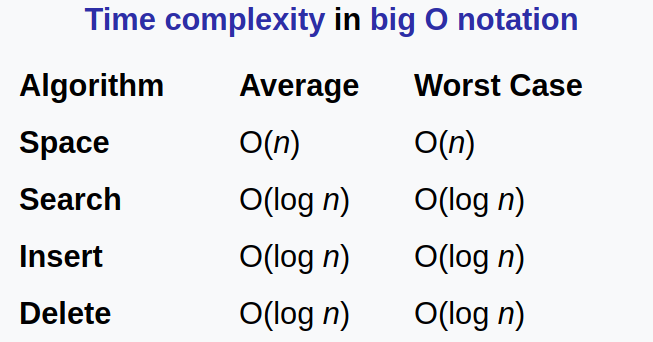
\includegraphics[width=1\textwidth]{./fig/23tree24.png}	
		\caption{Imagem retirada de [1] (vide \textit{Referências Bibliográficas})}
        \end{figure}
}

% \section[\thesection]{Terceiro Tópico}
% 
% \frame { \frametitle{Terceiro Tópico}
% 	\begin{block}{Tabelas}
% 		Qualquer recursos disponível no \texttt{LaTeX} e seus pacotes complementares podem ser utilizados, desde que ao 
% final a equipe gere um arquivo compactado (extensão .zip) contendo toda a ``\emph{pasta}'' com os \emph{slides} 
% desenvolvidos.
% 		\newline
% 		\newline
% 		A pasta gerada também deverá conter um arquivo \texttt{.pdf} com os \emph{slides} utilizados.
% 	\end{block}
% }
% 
% \frame { \frametitle{Terceiro Tópico}
% 	\begin{block}{Exemplo 01}
% 		Exemplos devem utilizar um \texttt{bloco} para serem apresentados, como o que está acontecendo neste momento, 
% ou seja, um bloco está sendo utilizado e seu título é \texttt{Exemplo 01}. 
% 		\newline
% 		\newline 
% 		Você também pode utilizar \textcolor{blue}{cores} para dar destaque no texto.
% 	\end{block}
% }
%
%---------------------------------------------------------------------------------------------------
% Questionário
%---------------------------------------------------------------------------------------------------
%
\section[\thesection]{Questionário}

\frame { \frametitle{Questionário}
	Deve haver, ao final, uma seção dedicada à apresentação de um questionário com pelo menos $05$ (cinco) questões, e 
suas respectivas respostas esperadas.
	\newline
	\newline
	Cada questão deverá ser um \texttt{bloco}, o mesmo ocorrendo com a resposta esperada.
	\newline
	\newline
	Veja o exemplo....
}

\frame { \frametitle{Questionário}
	\begin{block}{Questão 01}
	      Enunciado da primeira questão, se necessário com figuras, tabelas, e tudo mais.
	\end{block}
}	

\frame { \frametitle{Questionário}
	\begin{block}{Questão 01 -- Resposta Esperada}
	      Bloco com a resposta esperada para a primeira questão.
	\end{block}
}	
%
%---------------------------------------------------------------------------------------------------
% Referências Bibliográficas
%---------------------------------------------------------------------------------------------------
%
\section[\thesection]{Referências Bibliográficas}

%\frame { \frametitle{Referências Bibliográficas}
%	A última seção dos \emph{slides} deve apresentar as referências bibliográficas do trabalho: artigos, 
%\emph{websites}, livros, capítulos de livros, etc.
%	\newline
%	\newline
%	Veja o exemplo...
%}


\frame { \frametitle{Referências Bibliográficas}
	\begin{enumerate}
	 \item \url{https://pt.wikipedia.org/wiki/\%C3\%81rvore_2-3}
	 \item \url{https://www.passeidireto.com/disciplina/algoritmos-e-estrutura-de-dados-iii?type=6&materialid=1012744}
	 \item \url{https://www.ime.usp.br/~gold/cursos/2002/mac2301/aulas/b-arvore/b-arvore.html}
	 \item COOPER, K. and TORCZON, L. -- 2011 : \textit{Chapter 2 -- Scanners};
	 \item GRUNE, \textit{et al.} -- 2012 : \textit{Chapter 2 -- Program Text to Tokens -- 
Lexical Analysis}.
	\end{enumerate}
}

\frame { \frametitle{Referências Bibliográficas}
	Se desejar, pode encerrar com uma imagem, uma citação, etc.
	\begin{figure}[htbp]
		\centering
		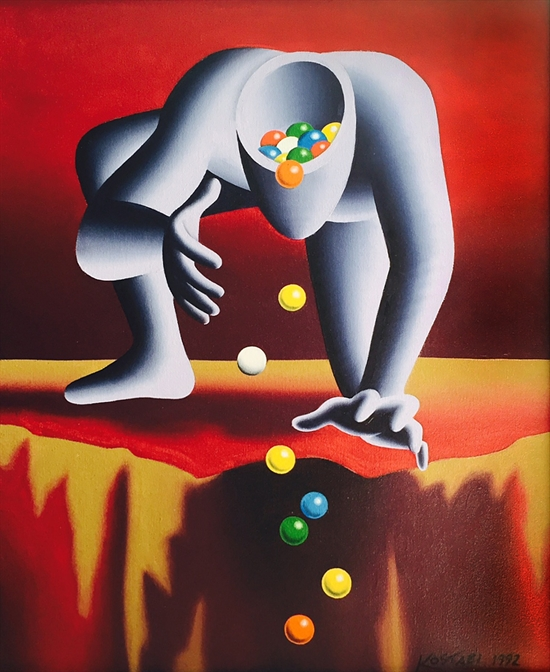
\includegraphics[width=0.50\textwidth]{./fig/MarkKostabi01.jpg}
		\caption{by Mark Kostabi.} 
\label{fig:traducaoRIparaLO}
   	\end{figure}
}

\end{document}
